\chapter{Fundamentação Técnica}\label{chp:LABEL_CASOS_DE_ESTUDOS}

Neste capítulo abortaremos o algoritmo de geração de \textit{isosupercícies} procedurais conhecido como Marching Cubes, escolhido para realizar a comparação entre os pipelines por se beneficiar das novas funcionalidades trazidas pelos mesh shader.

\section{O Algoritmo Marching Cubes}\label{sec:LABEL_CASOS_DE_ESTUDOS_SEC_A}

\begin{figure}
\centering
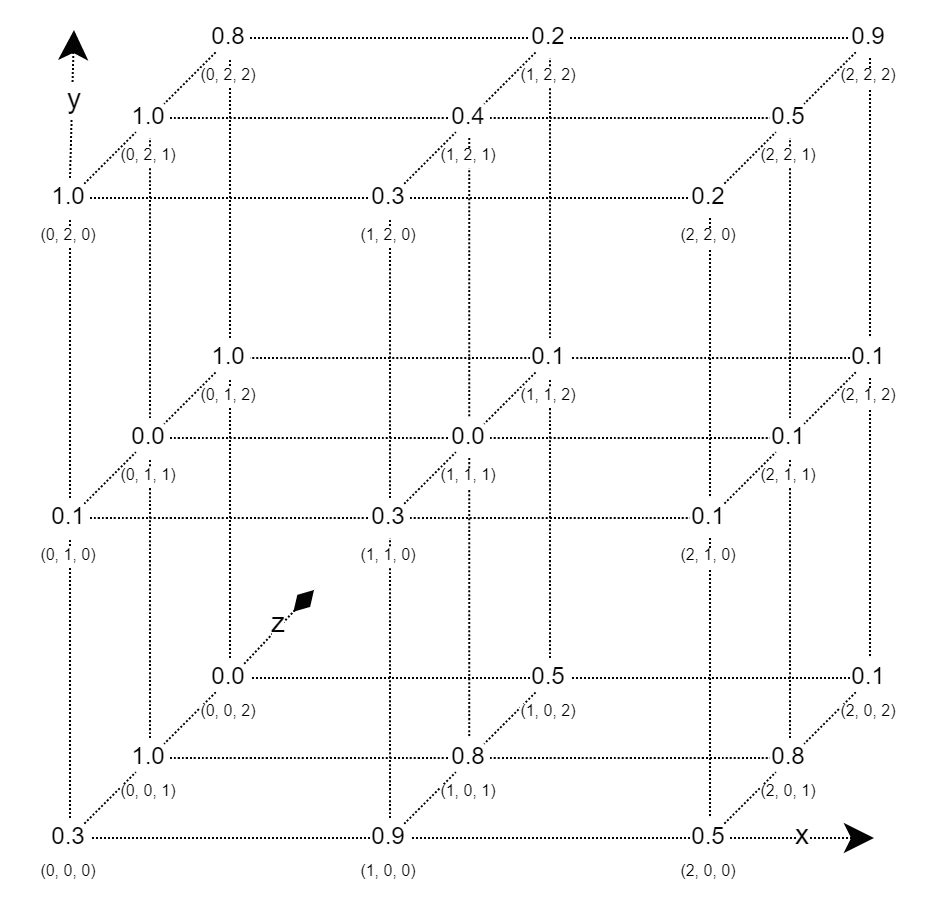
\includegraphics[width=0.6\textwidth]{imagens/MarchingCubes-NuvemDensidade.png}
\caption{Representação da densidade atribuída às coordenadas espaço}
\label{fig:LABEL_FIG_NUVEM_DENSIDADE}
\end{figure}

Proposto em 1987 para a visualização tridimensional dos resultados de exames de tomografias computadorizadas, Marching cubes \cite{REF_ART_MARCHING_CUBES} é um algoritmo capaz de construir superfícies de alta resolução utilizando uma abordagem de dividir para conquistar. Com o avanço na capacidade de processamento do hardware atual, o algoritmo obteve diversas outras usabilidades na área da computação gráfica. Como por exemplo no remapeamento na topologia de malhas complexas \cite{REF_ART_MARCHING_CUBES_REMESH} ou na geração dinâmica de terrenos proceduras em jogos eletrônicos \cite{REF_ART_MARCHING_CUBES_TERRAIN_GENERATION}.


Dado a representação volumétrica da superfície, denominada \textit{nuvem de pontos}, ilustrada pela Figura \ref{fig:LABEL_FIG_NUVEM_DENSIDADE}, o algoritmo percorre as sub sessões do espaço de interesse auxiliado por uma tabela de pesquisa chamada de \textit{tabela de triangularização}. A tabela de triangularização dita quais vértices serão conectados para formar os triângulos que irão compor a malha. Quanto menor for o tamanho das sub sessões, maior é a quantidade de triângulos construídos e, consequentemente, maior é o nível de detalhe da geometria final. 

Embora utilize apenas operações lógicas simples, marching cubes pode ser um algoritmo computacionalmente custoso quando requer um maior nível de detalhe da superfície. Visto que cada sub sessão pode ser percorrida individualmente, sua execução é altamente paralelizável. 

\section{Nuvem de pontos}\label{sec:LABEL_CASOS_DE_ESTUDOS_SEC_B}

A nuvem de pontos consiste em uma matriz cúbica de pontos. Um ponto é um vetor que possui duas informações: posição e densidade. Enquanto a primeira representa sua posição no espaço, a segunda armazena um valor entre 0 e 1 que é utilizado para determinar se aquele ponto está dentro ou fora da superfície. O \textit{nível da superfície} é um número constante $l$ que indica o valor mínimo de densidade necessária para um ponto estar dentro da superfície. Dado um ponto arbitrário p, diz-se que p está dentro da superfície se e somente se $densidade(p) \geq l$. Caso contrário, o ponto está fora da superfície.


Dado uma região no espaço tridimensional, a construção da nuvem de pontos se dá ao distribuir pontos em intervalos regulares dentro desta região. Visando manter as proporções da malha pelas 3 dimensões em 1:1:1, deve-se atribuir a mesma quantidade de pontos igualmente entre elas. Com os pontos distribuídos, aplica-se para cada ponto, uma função $f$ tal que $f(x, y, z) => d$, onde $x$, $y$ e $z$ são as coordenadas do ponto no espaço e $d$ é a densidade atribuída a aquele ponto. A disposição de densidades no espaço junto do nível da superfície ditam a silhueta da geometria que será construída.

\section{Geração dos Triângulos}\label{sec:LABEL_CASOS_DE_ESTUDOS_SEC_C}

\begin{figure}
\centering
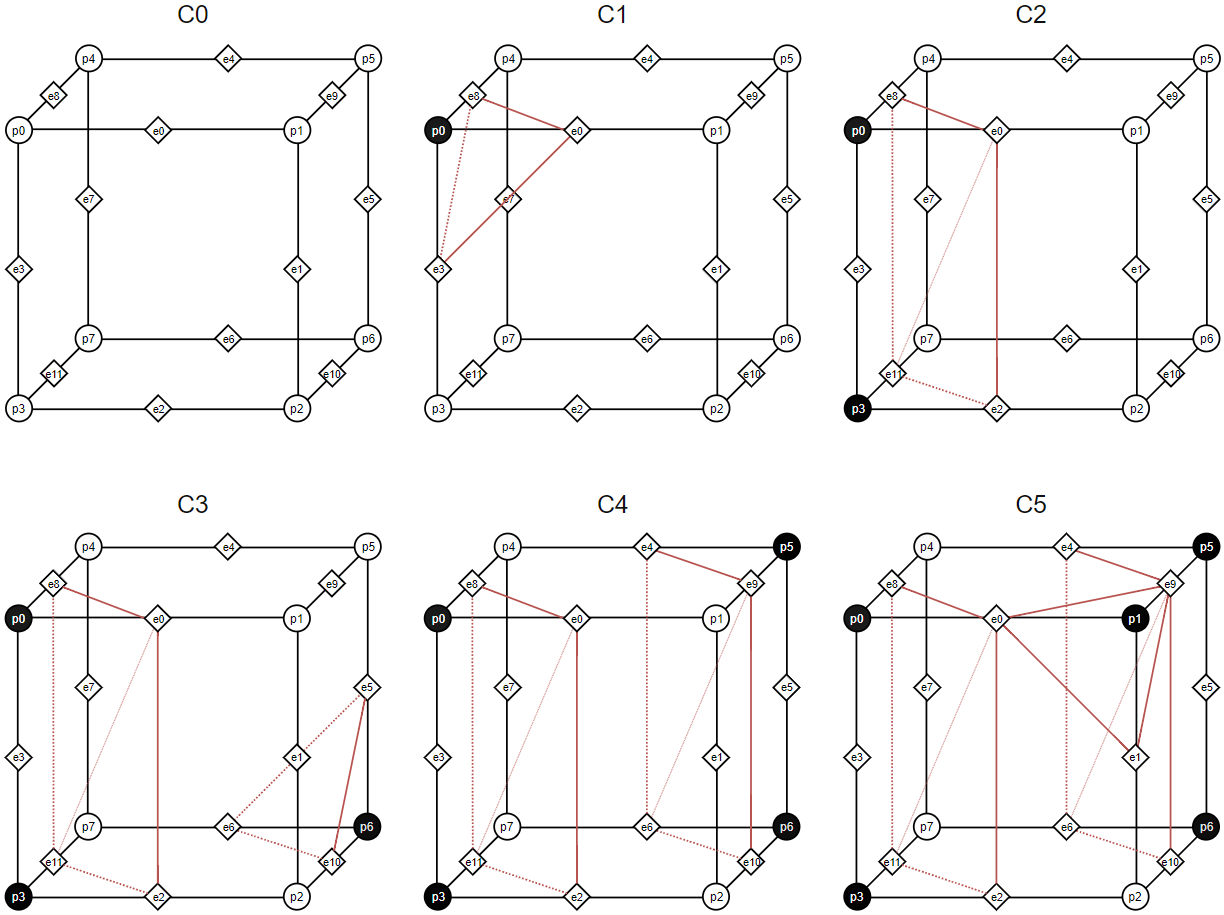
\includegraphics[width=0.9\textwidth]{imagens/MC-ConfiguracoesCubo.png}
\caption{Representação das distintas configurações de cubo}
\label{fig:LABEL_FIG_CONFIGURACOES_CUBO}
\end{figure}

Após a construção da nuvem de pontos, os pontos presentes nesta são agrupados 8 a 8, de forma que cada ponto represente a vértice de um cubo com arestas de tamanho máximo $k$, onde $k$ é a distancia entre dois pontos vizinhos arbitrários na nuvem de pontos. Para cada cubo gerado, verifica-se a configuração dos pontos que o representa. O objetivo do algoritmo é construir triângulos que separem os pontos que estão fora da superfície dos que estão dentro.

Visto o exemplo ilustrado na figura \ref{fig:LABEL_FIG_CONFIGURACOES_CUBO}, a configuração $C0$ não apresenta nenhum ponto dentro da superfície, logo não necessita da criação de triângulos. Já em $C1$, o ponto $p1$ é indicado como dentro da superfície, então um triangulo é gerado conectando as arestas $e0$, $e3$ e $e8$. Em $C2$, além de $p1$, $p3$ também está fora da superfície, então são construídos dois triângulos: o triangulo $e0$, $e8$ e $e11$ e o triangulo $e0$, $e2$ e $e11$. Considerando que cada ponto contém apenas duas possibilidades de estados: dentro ou fora da superfície e que um cubo é composto por 8 pontos, existem um total de $2^8 = 256$ possibilidades distintas de triangularização. Entretanto, apenas 14 dessas são configurações únicas, sendo o restante apenas variações de rotação destas. Para auxiliar a tarefa de construção dos triângulos, o algoritmo de marching cubes utiliza de uma tabela de pesquisa. Cada linha desta tabela representa uma configuração distinta de cubo e indica quais arestas devem ser conectadas para formar um triangulo.

Afim de se construir geometrias mais \textit{aredondadas}, incrementando seu nível de detalhe, a posição das vértices dos triângulos é interpolada de acordo com a densidade dos pontos que a representam. Dado dois pontos adjacentes $p0$ e $p1$, suas respectivas posições no espaço $\overrightarrow{P0}$ e $\overrightarrow{P1}$ e o nível da superfície $l$, a posição $\overrightarrow{P}$ do vértice do triangulo construído sob a aresta que os intercepta se da pela seguinte formula:


\begin{equation}
    \overrightarrow{P} = \overrightarrow{P0} + \frac{l - densidade(p0)}{densidade(p1) - densidade(p0)} * (\overrightarrow{P0} - \overrightarrow{P1})
\end{equation}

A Figura \ref{fig:LABEL_FIG_INTERPOLACAO} ilustra a diferença visual obtida através dessa melhoria.

\begin{figure}
\centering
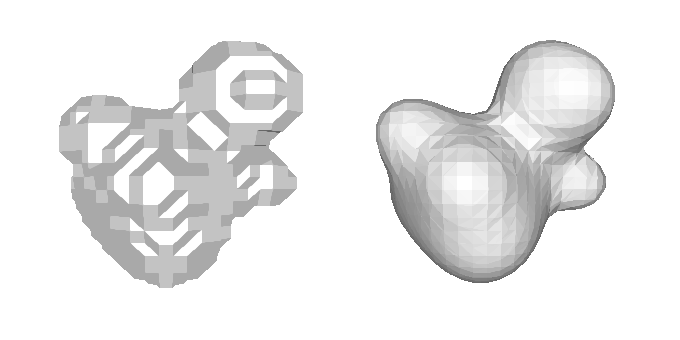
\includegraphics[width=0.6\textwidth]{imagens/PontoMedioXInterpolado.png}
\caption{Malha interpolada pelo ponto médio dos vértices (à esquerda) e sua representação interpolada pela média de densidade dos pontos adjacentes (à direita) }
\label{fig:LABEL_FIG_INTERPOLACAO}
\end{figure}

Conforme ilustrado na figura \ref{fig:LABEL_FIG_EXECUCAO_ALGORITIMO}, o algoritmo então marcha por todos os possíveis cubos presentes no espaço adicionando os vértices criados a uma lista de vértices e índices que serão repassados para o pipeline de rasterização posteriormente.

\begin{figure}
\centering
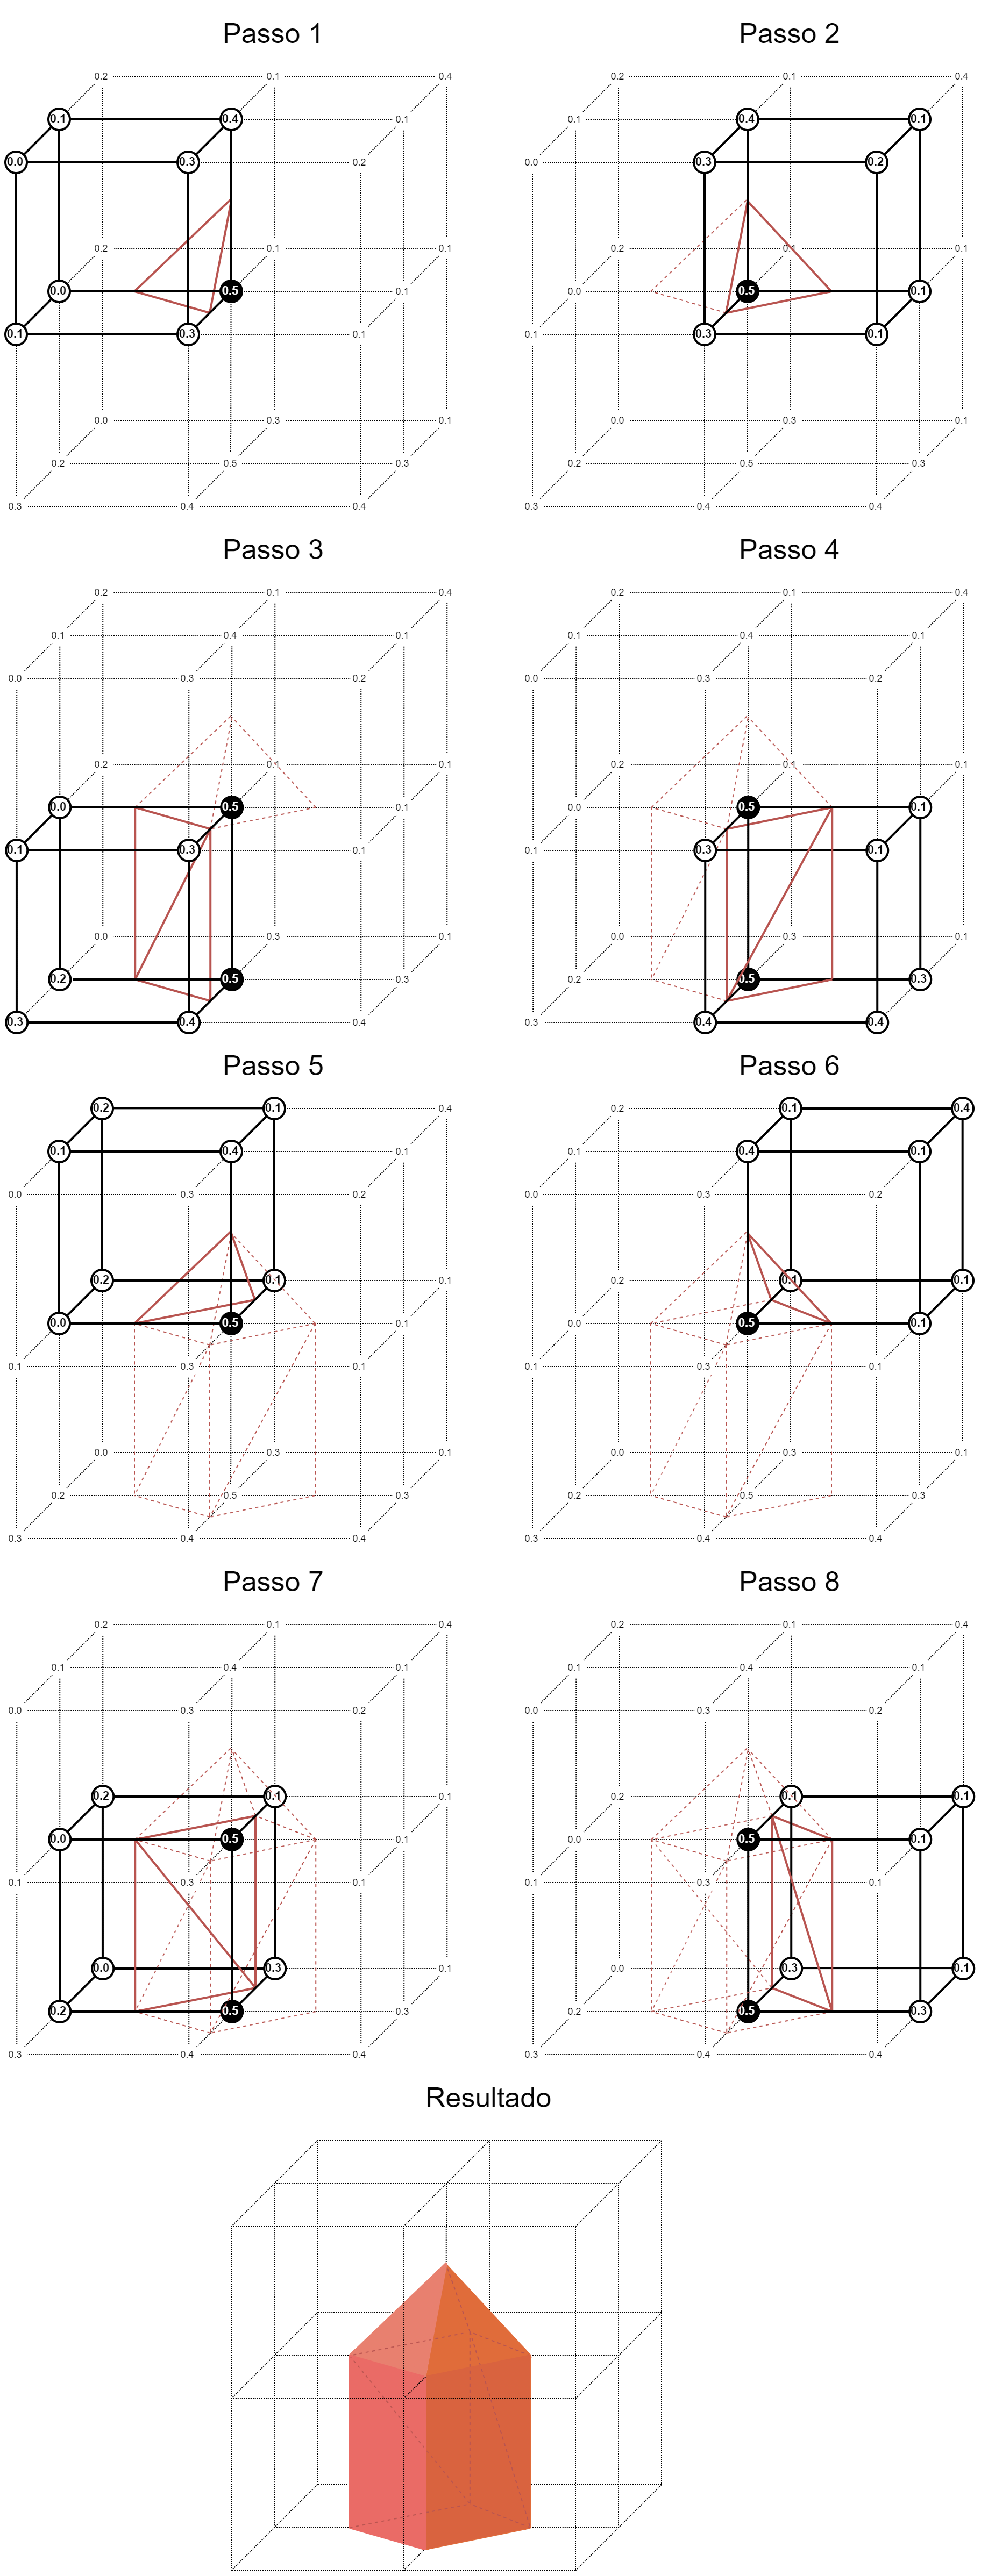
\includegraphics[width=0.6\textwidth]{imagens/MarchingCubes-Execucao.png}
\caption{Passo a passo da execução do algorítimo de marching cubes}
\label{fig:LABEL_FIG_EXECUCAO_ALGORITIMO}
\end{figure}

\section{Complexidade}\label{sec:LABEL_CASOS_DE_ESTUDOS_SEC_D}

Cado a natureza cúbica da nuvem de pontos, a quantidade de interações cresce na terceira potencia. Uma nuvem contendo 2 pontos em cada dimensão possuí um total de 8 pontos. Neste caso, apenas um cubo pode ser formado, então o algorítimo executará apenas uma interação. Caso incrementemos um 1 ponto em cada dimensão esta nuvem possuirá então 27 pontos no total, podendo agora formar 8 cubos distintos. Logo, 8 interações são executadas. Dado uma nuvem cúbica com $n$ pontos distribuídos uniformemente nas 3 dimensões, temos que a quantidade de pontos presentes nesta se por $n ^ 3$. Já a quantidade de cubos formados é definida por $\lfloor\frac{n ^ 3}{8}\rfloor$. Com isto, observamos que a complexidade do algoritmo de marching cubes é da ordem de $\mathcal{O}(n^3)$

Considerando uma região de interesse no espaço de $10m^3$, caso deseja-se construir uma isosuperfície com precisão de $1m$, deve-se distribuir $10$ pontos distanciados igualitariamente entre as 3 dimensões dentro deste intervalo. Dependendo da distribuição de densidade dos pontos, conforme exemplificado em \ref{sec:LABEL_CASOS_DE_ESTUDOS_SEC_B}, múltiplas combinações de triangularizações podem ser geradas. Embora não seja trivial de visualizar, a combinação de triangularização mais complexa contém um total de 5 triângulos. Tomando esse como pior dos casos, podemos estimar que a quantidade máxima triângulos com 10 pontos é de $10^3*5 = 5000$ triângulos.

\begin{figure}
\centering
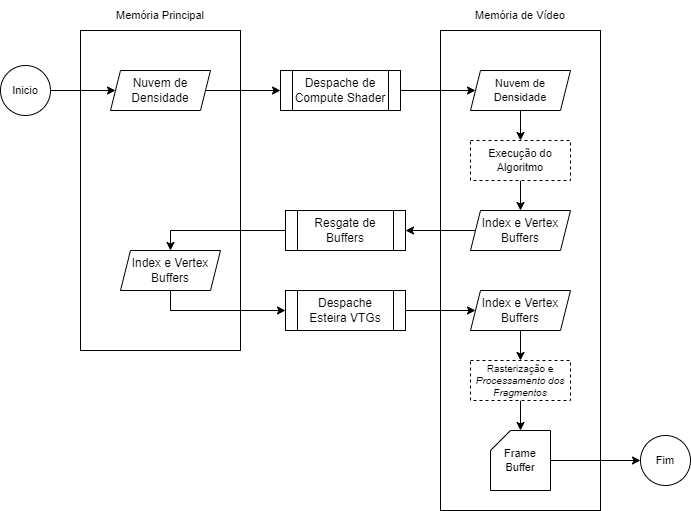
\includegraphics[width=0.9\textwidth]{imagens/FluxoDados-RendIndireta.drawio.png}
\caption{Fluxograma dos dados em renderização indireta}
\label{fig:LABEL_FIG_REND_INDIRETA}
\end{figure}

\section{Implementações}\label{sec:LABEL_FLUXO_DOS_DADOS}

O algoritmo de marching cubes pode ser implementado de forma eficiente em duas distintas configurações: renderização indireta através de compute shaders ou renderização direta com mesh shaders.

Conforme comentado na Sessão \ref{sec:LABEL_RENDERIZACAO_INDIRETA}, os dados processados com compute shaders devem ser renderizados de forma indireta. A Figura \ref{fig:LABEL_FIG_REND_INDIRETA} ilustra a sequencia de etapas necessárias para a implementação do marching cubes. O fluxo inicia-se com a pré-montagem da nuvem de densidades da geometria a ser renderizada. Após o despache do compute shader, a nuvem de dados é armazenada em um SSBO. Após a execução do algoritmo, os index e vertex buffers gerados são armazenados em um segundo SSBO que pode ser resgatado através de uma chamada a API gráfica. Como compute shaders não se comunicam com o fluxo de renderização, os dados computados por ele devem retornar a memória principal antes de serem tramitados para um programa de renderização VGTs.

Já no segundo fluxo, ilustrado pela figura \ref{fig:LABEL_FIG_REND_DIRETA}, temos uma sequencia mais otimizada. Após a execução do algoritmo de marching cubes, os index e vertex buffers são repassados diretamente para a rasterização, onde são fragmentados sem a necessidade de retornar a memória principal.

\begin{figure}
\centering
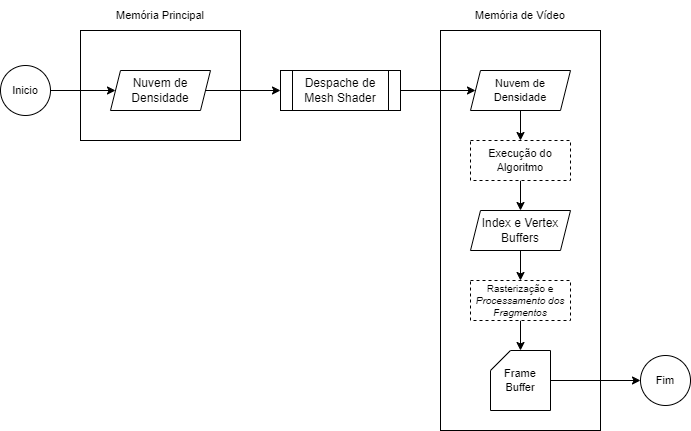
\includegraphics[width=1\textwidth]{imagens/FluxoDados-RendDireta.drawio.png}
\caption{Fluxograma dos dados em renderização direta}
\label{fig:LABEL_FIG_REND_DIRETA}
\end{figure}